\documentclass[9pt,twoside,lineno]{pnas-new}
\usepackage{rotating}
\usepackage{multirow}
\templatetype{pnassupportinginfo}

\title{High geomagnetic field intensity recorded by anorthosite xenoliths requires a vigorous late Mesoproterozoic geodynamo}
\author{Yiming Zhang, Nicholas L. Swanson-Hysell, Margaret S. Avery, Roger R. Fu}
\correspondingauthor{Yiming Zhang\\E-mail: yimingzhang@berkeley.edu}

\begin{document}

\maketitle

% \begin{figure*}[h!]
% \noindent\includegraphics[width=0.8\textwidth]{Petro_QDM_SI.png}
% \centering
% \caption{{Petrographic images and magnetic images from the main manuscript with additional anisotropy experiment results. In A-F, we show that the Beaver River anorthosite often lack large oxide needles within plagioclase crystals carrying strong magnetic remanence  differences of magnetic carriers which is in contrast to what is seen in Duluth Complex anorthosites. E-H show an experiment performed on both anorthosite xenoliths where we apply a first field along the y axis of the field of view and then apply a second field of 300 mT orthogonal to the first field direction. The isothermal remanent magnetizations acquired by both anorthosites were imaged with a quantum diamond microscope after the application of each field. The magnetic images show that dipole-like remanent magnetizations of Beaver River anorthosite align well with the first applied field direction and rotated to align with the second applied field direction with little anisotropic behavior. In contrast, the remanence magnetizations carried by the magnetic needles in plagioclase 1 of the Duluth anorthosite xenolith align well with the first applied field but those in plagioclase 2 tend to acquire an oblique remanence direction with respect to the field direction (F). After the application of a 300 mT external field, magnetization of those needles in plagioclase 1 did not reverse due to strong shape anisotropy whereas those needles in plagioclase 2 reversed but still acquired remanence oblique to the field direction. This experiments illustrates that the Beaver River anorthosite xenolith has much lower degrees of magnetic anisotropy than the Duluth anorthosite xenolith. B$_z$ denotes magnetic field intensity in the vertical direction with positive values corresponding to the out of page direction.  }}
% \label{fig:Petro_QDM_SI}
% \end{figure*}
% \clearpage


\begin{figure*}[h!]
\noindent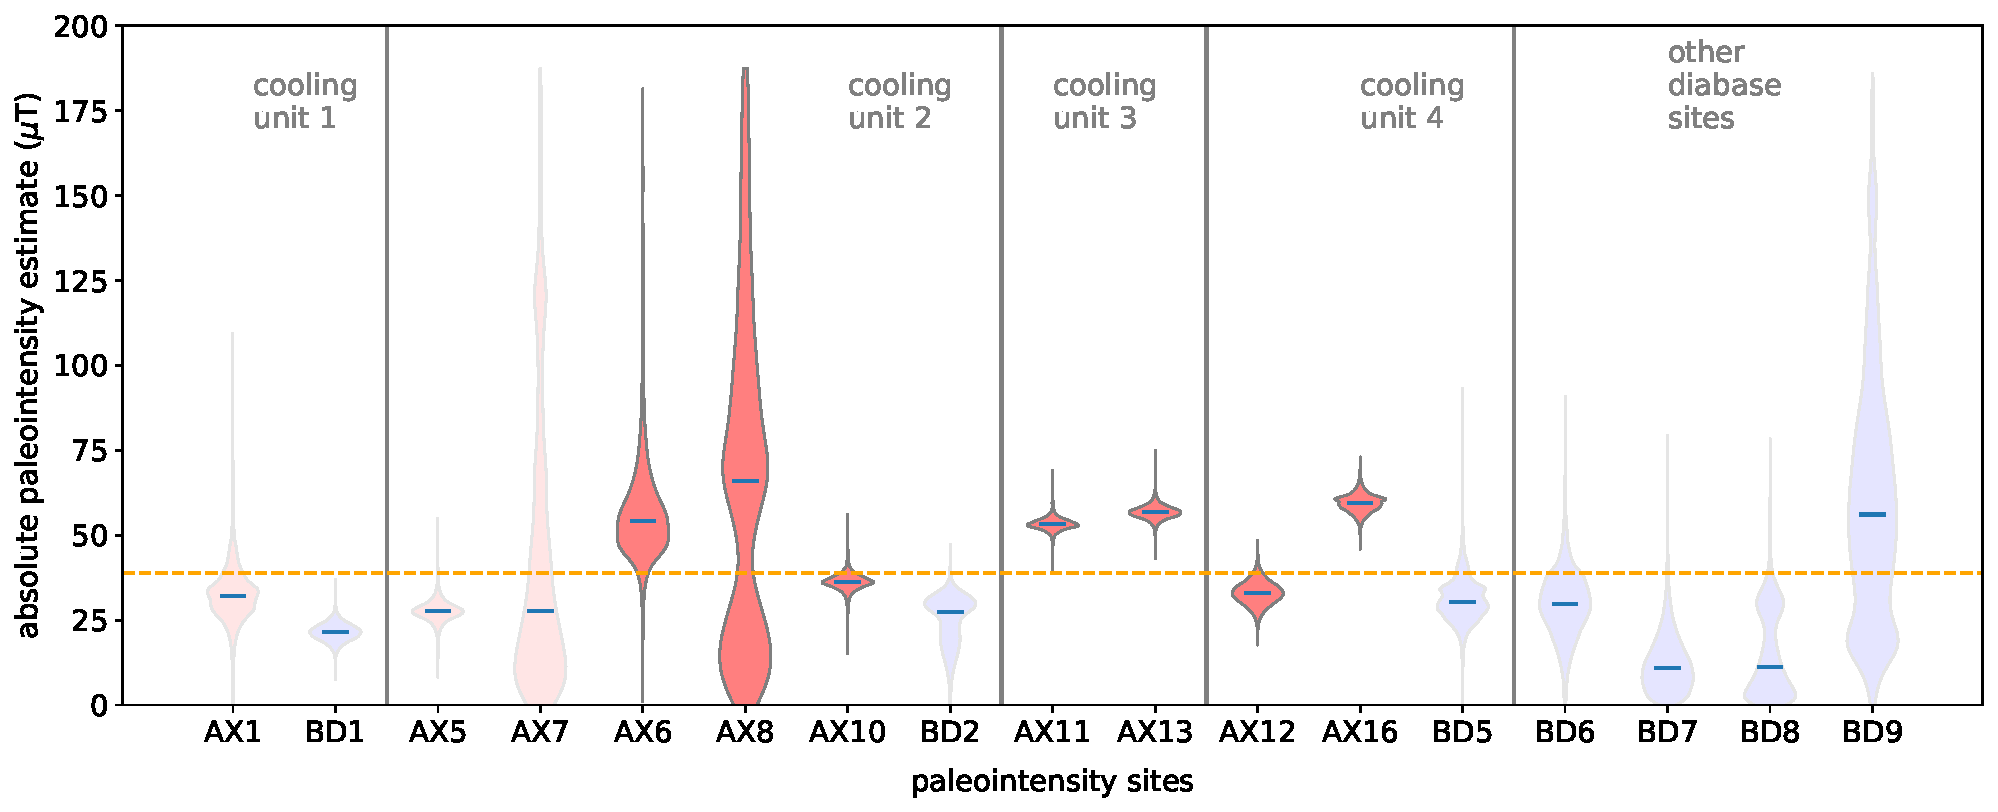
\includegraphics[width=17.8 cm]{PINT_BiCEP.pdf}
\centering
\caption{{Violin plots of site-level posterior paleointensity distributions estimated using the bias corrected estimation of paleointensity (BiCEP) method developed by \citealp{Cych2021a}. Assuming that paleointensity estimates from specimens that come from a same cooling unit are distributed around a true paleointensity value with the various deflections being expressed as the curvature parameter of the NRM/TRM plot \cite{Arai1963a, Paterson2011a}, the method uses all paleointensity measurement-level data without applying selection criteria. For comparison of results from this independent method with those based on our selection (as show in Fig. 4 in manuscript), we highlight the anorthosite sites that pass our paleointensity selection and make other anorthosite and diabase transparent. The results from the BiCEP method address the uncertainties associated with anorthosite AX6 and AX8. This is associated with the relatively variable specimen behaviors within these two sites. But for sites AX10, AX11, AX13, AX12, and AX16, the posterior probability distributions have very narrow bounds, consistent with the interpretation that these anorthosites are faithful paleointensity recorders that have high-quality paleointensity behaviors. }}
\label{fig:PINT_BiCEP}
\end{figure*}

\clearpage

\begin{figure}
\noindent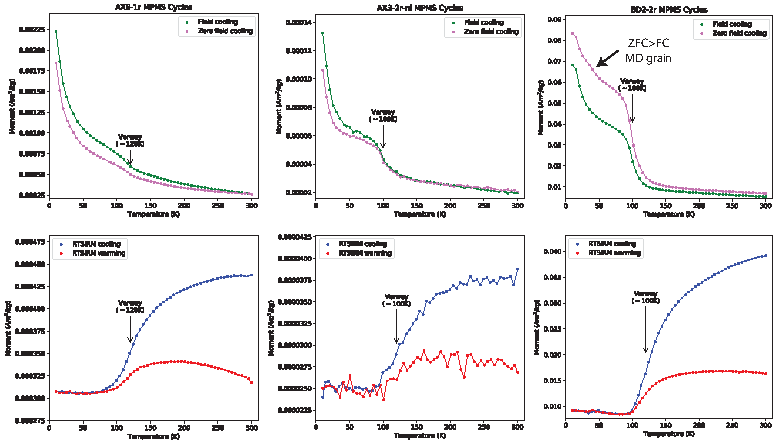
\includegraphics[width=\textwidth]{MPMS.pdf}
\centering
\caption{{Low-temperature magnetic property measurement system (MPMS) experiment results. In the field-cooled (FC) experiments, the magnetization was measured upon warming following the specimen having cooled in an applied field of 2.5 T from 300 to 10 K. In the zero-field-cooled (ZFC) experiment, a low-temperature saturation isothermal remanence (LTSIRM) of 2.5 T was applied at 10 K after the specimen cooled in a (near-)zero field. In the room-temperature saturation isothermal remanence (RTSIRM) experiment, the sample was pulsed with a 2.5 T field at room temperature ($\sim$300 K) and then cooled to 10 K and warmed back to room temperature in a (near-) zero field. Specimen AX6-1r is from anorthosite AX6 which passed our paleointensity selection. It has a well-defined Verwey transition $\sim$120 K \cite{Verwey1939a}. Specimens AX3-2r-ni and BD2-2r show Verwey transition but the transition temperatures are suppressed below $\sim$120 K. Specimen BD2-2r has a consistently higher moment during the zero-field-cooled step than during the field-cooled step. This is consistent with the interpretation that multidomian magnetic carriers exist in significant quantity in this specimen.}}
\label{fig:MPMS}
\end{figure}

\clearpage

\begin{figure*}[h!]
\noindent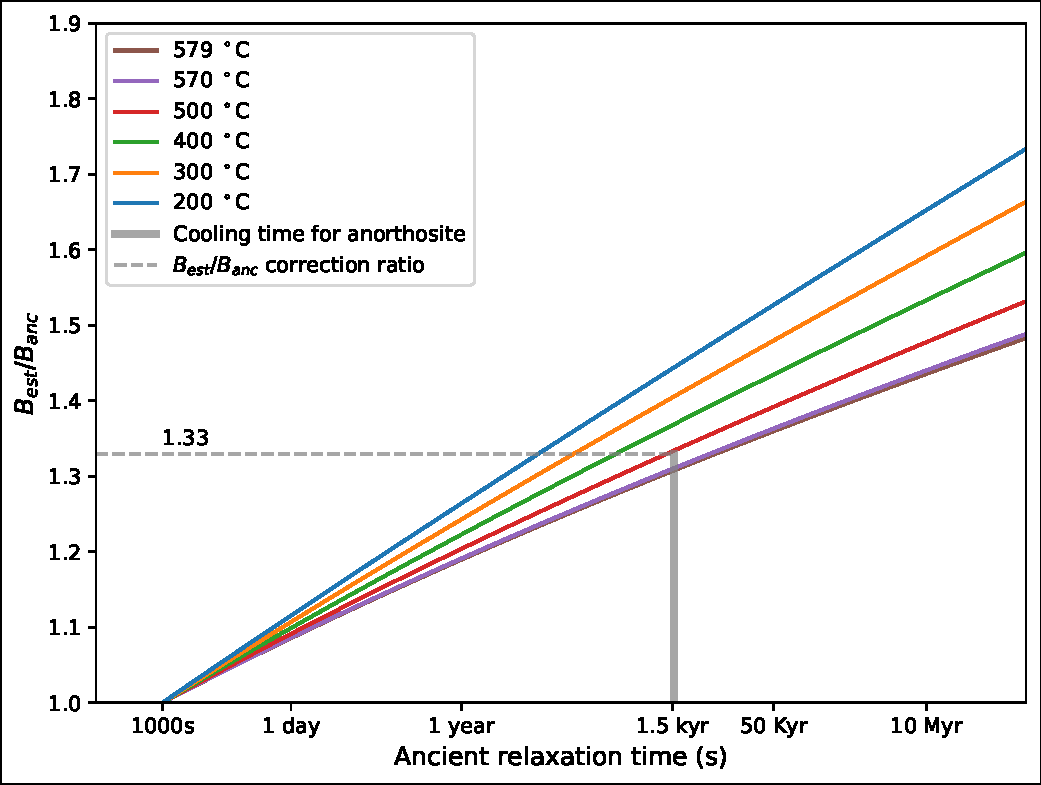
\includegraphics[width=17.8 cm]{Cooling_rate_correction.pdf}
\centering
\caption{{Graph of predicted paleointensity overestimate due to slow cooling of the intrusive Beaver River diabase and anorthosite xenoliths relative to the cooling rate in laboratory following the model of \citealp{Halgedahl1980a}. Because the majority of the anorthosites have unblocking temperatures between 500\textdegree C and 580\textdegree C, we estimate that the slow cooling during natural remanence acquisition could have resulted in a 36\% overestimate. Thus, a correction factor of 0.74 is applied at specimen level for the paleointensity summary plot.}}
\label{fig:PINT_cooling_corrected}
\end{figure*}

\clearpage

\begin{figure*}[h!]
\noindent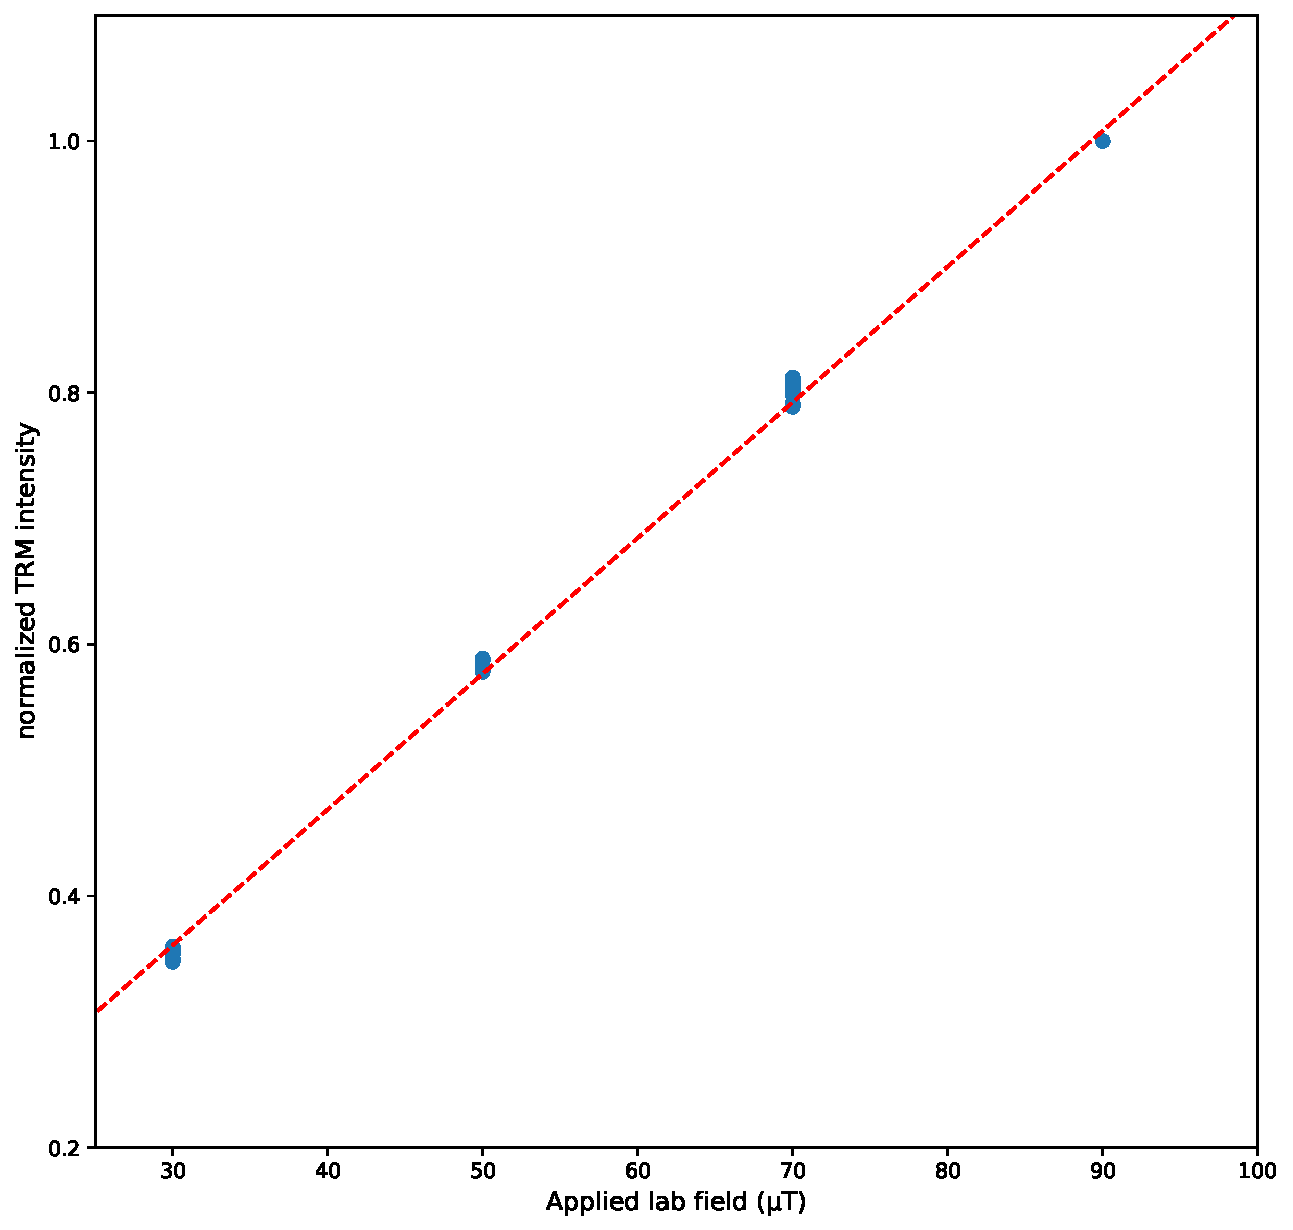
\includegraphics[width=0.9\textwidth]{Linear_TRM_test.pdf}
\centering
\caption{{Plot of linear thermal remanent magnetization acquisition experiment results. After IZZI-type Thellier paleointensity experiments, full TRMs were imparted on the same specimens in known lab fields of 30, 50, 70, and 90 $\mu$T. The red dashed line shows a linear fit through the data points. The results show that the anorthosite xenoliths do not acquire saturation remanence or display non-linear remanence acquisition under fields relevant to this study. Therefore, non-linear acquisition correction is not needed for our paleointensity results. }}
\label{fig:nonlinear_check}
\end{figure*}


%To check for nonlinear acqusition, we applied full TRMs to a set of anorthosite specimens with lab fields of 30, 50, 70, and 90 $\mu$T along specimen vertical axes. The results show that these anorthosite specimens did not saturate upon the applied fields and there is thus no need for correcting nonlinear thermal remanence acquisitions (\citealp{Selkin2007a}; Fig. S4). 

\clearpage

\begin{figure*}[h!]
\noindent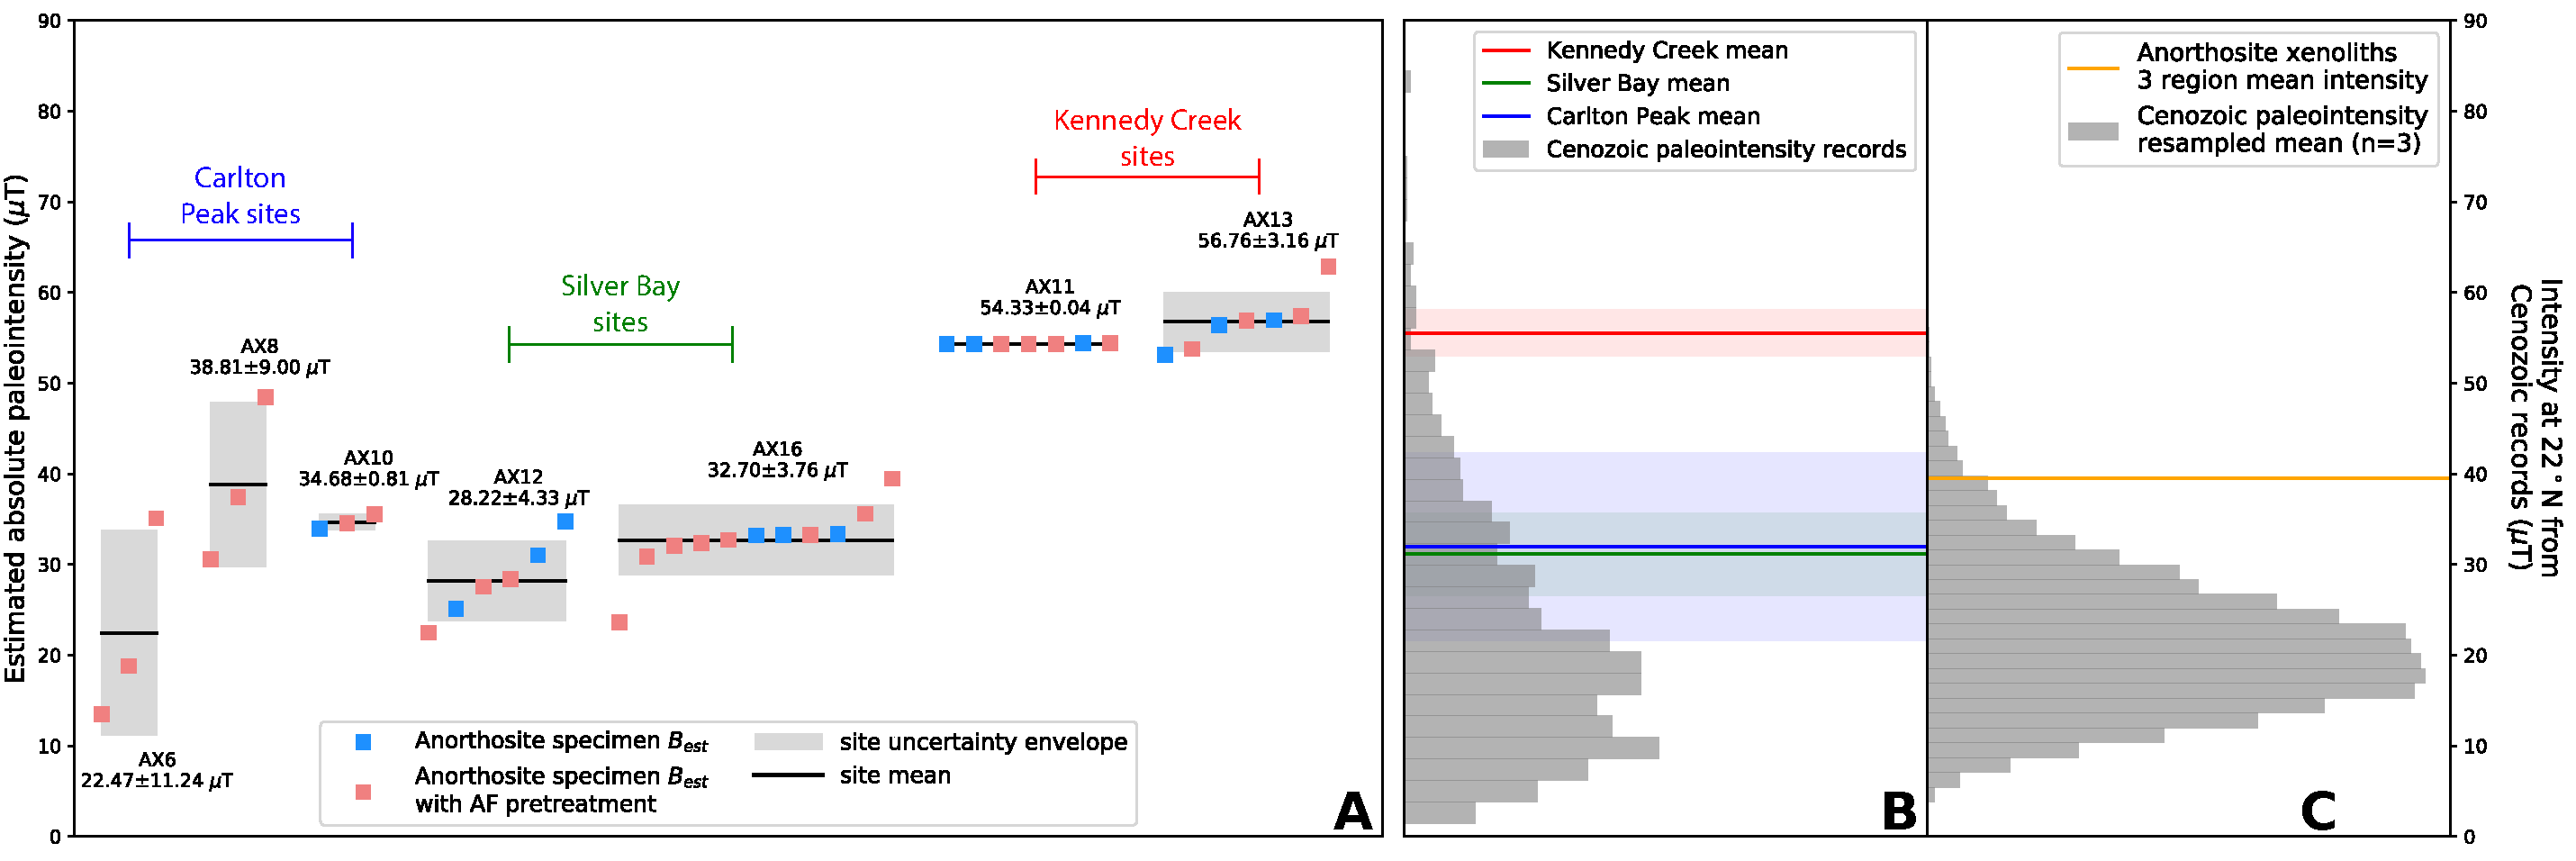
\includegraphics[width=0.9\textwidth]{Cenozoic_resample_SI.pdf}
\centering
\caption{\footnotesize{A) Summary plot of individual specimen absolute paleointensity results (square symbols) and their averages and standard deviations at site level (black bars with grey uncertainty boxes) from this study. All results are corrected for cooling rate with a factor of 0.74. Each `AX' site is an individual anorthosite xenolith within the Beaver River diabase. The sites with successful experiments come from 3 regions which would have cooled at distinct times yielding similar estimates within the each region with differences between regions. B) Specimen level means calculated for these regions are compared to the distribution of intensities calculated from the existing paleointensity data in the PINT database (PINT v8.0.0; \url{http://www.pintdb.org/}; \citealp{Bono2021a}) at the latitude corresponding to the paleolatitude of study region (22\textdegree N). C) The mean of the 3 regional means is compared to means calculated from 3 random values drawn from the Cenozoic data. The paleointensity records used for resampling are filtered for Q$_{PI} \geq$3 \cite{Biggin2014a}. The distribution represents a total of 10,000 iterations of taking 3 random draws and calculating the mean.}}
\label{fig:Cenozoic_PINT}
\end{figure*}


\clearpage

\begin{sidewaystable}
\caption{\footnotesize{Specimen paleointensity results that passed our selection. Paleointensity results for specimens that passed quality criteria. B$_{anc}$ is the calculated ancient field intensity over the chosen temperature interval in $\mu$T. T$_{min}$ and T$_{max}$ indicate the temperature interval over which the best fit for paleointensity was defined. N is the number of steps used within the selected interval for paleointensity determination. FRAC is the fraction of remanence. NpTRM shows the number of pTRM checks within the selected interval for paleointensity determination. $\beta$ is the scatter parameter.  GAP-MAX is the maximum magnetization gap between two adjacent steps. MAD is the maximum angle of deviation. DANG is the deviation angle. SCAT is the scatter parameter. Paleolatitude is calculated from the inclination values reported in \cite{Zhang2021b}. $\gamma$ is the gamma statistic that measures the angle between the last pTRM step used for paleointensity determination and the applied field direction. V(A)DM is the virtual (axial) dipole moment reported in $10^{21}$Am$^2$ (ZAm$^2$). }}
\centering
\begin{tabular}{cccccccccccccccc}
\hline
Site & Specimen & B$_{anc}$ & T$_{min}$ & T$_{max}$ & N    & FRAC & NpTRM & $\beta$ & GAP-MAX & MAD ($^\circ$) & DANG ($^\circ$) & SCAT & Paleolatitude & $\gamma$ & VADM (ZAm$^2$) \\
\hline
AX6  & AX6-2a   & 18.25     & 400       & 585       & 18 & 0.7  & 10    & 0.04    & 0.12    & 3.44           & 3.43            & PASS & 21.97         & 2.7      & 29.34         \\
AX6  & AX6-3a   & 25.39     & 400       & 585       & 18 & 0.76 & 10    & 0.04    & 0.1     & 4.28           & 2.88            & PASS & 21.97         & 3.2      & 40.82         \\
AX6  & AX6-1a   & 47.36     & 475       & 585       & 15 & 0.6  & 10    & 0.02    & 0.16    & 2.92           & 1.67            & PASS & 21.97         & 2        & 76.13         \\
AX8  & AX8-3a   & 41.3      & 400       & 580       & 17 & 0.75 & 9     & 0.03    & 0.14    & 4.38           & 2.22            & PASS & 22.98         & 11.2     & 65.53         \\
AX8  & AX8-2a   & 50.51     & 400       & 580       & 17 & 0.63 & 9     & 0.04    & 0.16    & 3.19           & 1.29            & PASS & 22.98         & 3.7      & 80.15         \\
AX8  & AX8-1a   & 65.38     & 425       & 566       & 13 & 0.6  & 8     & 0.07    & 0.2     & 5.28           & 2.95            & PASS & 22.98         & 7        & 103.74        \\
AX10 & AX10-1a  & 45.84     & 425       & 585       & 17 & 0.78 & 10    & 0.06    & 0.24    & 5.6            & 2.62            & PASS & 20.37         & 4.7      & 75.2          \\
AX10 & AX10-2a  & 46.61     & 450       & 585       & 16 & 0.62 & 10    & 0.04    & 0.2     & 5.32           & 2.24            & PASS & 20.37         & 7.8      & 76.46         \\
AX10 & AX10-3a  & 48.01     & 425       & 585       & 17 & 0.69 & 10    & 0.04    & 0.24    & 4.02           & 1.56            & PASS & 20.37         & 5.8      & 78.76         \\
AX11 & AX11-1a  & 73.29     & 425       & 560       & 10 & 0.67 & 6     & 0.08    & 0.21    & 5.28           & 2.54            & PASS & 19.43         & 5.9      & 121.64        \\
AX11 & AX11-2a  & 73.29     & 400       & 560       & 11 & 0.65 & 6     & 0.07    & 0.21    & 3.94           & 1.51            & PASS & 19.43         & 9.9      & 121.64        \\
AX11 & AX11-4a  & 73.31     & 500       & 570       & 11 & 0.66 & 8     & 0.09    & 0.2     & 1.53           & 3.27            & PASS & 19.43         & 5.6      & 121.68        \\
AX11 & AX11-6a  & 73.32     & 200       & 562       & 14 & 0.69 & 7     & 0.07    & 0.17    & 4              & 1.33            & PASS & 19.43         & 3        & 121.69        \\
AX11 & AX11-9a  & 73.34     & 100       & 562       & 15 & 0.67 & 7     & 0.06    & 0.17    & 5.34           & 1.13            & PASS & 19.43         & 11.9     & 121.73        \\
AX11 & AX11-3a  & 73.41     & 400       & 560       & 11 & 0.66 & 6     & 0.08    & 0.21    & 3.95           & 2.11            & PASS & 19.43         & 8.2      & 121.84        \\
AX11 & AX11-5a  & 73.44     & 400       & 566       & 14 & 0.73 & 8     & 0.05    & 0.18    & 2.93           & 0.85            & PASS & 19.43         & 1.9      & 121.89        \\
AX12 & AX12-14a & 30.34     & 475       & 585       & 16 & 0.75 & 10    & 0.06    & 0.17    & 1.74           & 0.55            & PASS & 35.73         & 0.9      & 40.86         \\
AX12 & AX12-1a  & 33.89     & 0         & 580       & 21 & 0.97 & 9     & 0.03    & 0.17    & 5.47           & 4.73            & PASS & 35.73         & 10       & 45.64         \\
AX12 & AX12-6a  & 37.18     & 425       & 564       & 12 & 0.69 & 7     & 0.08    & 0.22    & 3.64           & 2.05            & PASS & 35.73         & 5        & 50.07         \\
AX12 & AX12-8a  & 38.34     & 475       & 565       & 12 & 0.75 & 8     & 0.06    & 0.25    & 1.46           & 2.29            & PASS & 35.73         & 1.6      & 51.63         \\
AX12 & AX12-4a  & 41.89     & 500       & 585       & 14 & 0.66 & 10    & 0.05    & 0.24    & 3.85           & 3.19            & PASS & 35.73         & 11.4     & 56.42         \\
AX12 & AX12-2a  & 46.94     & 425       & 570       & 14 & 0.7  & 8     & 0.05    & 0.24    & 3.39           & 2.38            & PASS & 35.73         & 7        & 63.22         \\
AX13 & AX13-3a  & 71.68     & 100       & 550       & 12 & 0.71 & 5     & 0.08    & 0.22    & 5.92           & 1.88            & PASS & 19.36         & 3.4      & 119.07        \\
AX13 & AX13-7a  & 72.6      & 475       & 585       & 15 & 0.61 & 10    & 0.03    & 0.2     & 3.62           & 2.09            & PASS & 19.36         & 11.6     & 120.6         \\
AX13 & AX13-4a  & 76.13     & 200       & 550       & 11 & 0.65 & 5     & 0.04    & 0.18    & 8.82           & 1.07            & PASS & 19.36         & 3.7      & 126.47        \\
AX13 & AX13-6a  & 76.8      & 200       & 555       & 12 & 0.7  & 6     & 0.06    & 0.22    & 3.82           & 1.53            & PASS & 19.36         & 4.5      & 127.58        \\
AX13 & AX13-2a  & 76.86     & 200       & 555       & 12 & 0.71 & 6     & 0.05    & 0.2     & 8.08           & 2.23            & PASS & 19.36         & 4.1      & 127.68        \\
AX13 & AX13-9a  & 77.48     & 0         & 564       & 17 & 0.94 & 7     & 0.03    & 0.16    & 5.96           & 1.07            & PASS & 19.36         & 2.6      & 128.71        \\
AX13 & AX13-8a  & 84.83     & 450       & 570       & 13 & 0.81 & 8     & 0.02    & 0.24    & 3.69           & 1.82            & PASS & 19.36         & 5.1      & 140.92        \\
AX16 & AX16-15a & 31.91     & 475       & 570       & 13 & 0.61 & 8     & 0.07    & 0.17    & 3.07           & 1.41            & PASS & 30.08         & 2.6      & 46.16         \\
AX16 & AX16-13a & 41.68     & 400       & 570       & 15 & 0.72 & 8     & 0.07    & 0.2     & 3.47           & 1.85            & PASS & 30.08         & 1.1      & 60.29         \\
AX16 & AX16-16a & 43.3      & 400       & 562       & 13 & 0.65 & 7     & 0.09    & 0.18    & 5.14           & 2.94            & PASS & 30.08         & 2        & 62.63         \\
AX16 & AX16-14a & 43.64     & 400       & 565       & 14 & 0.63 & 8     & 0.08    & 0.14    & 3.84           & 2.12            & PASS & 30.08         & 6        & 63.13         \\
AX16 & AX16-11a & 44.17     & 450       & 570       & 14 & 0.7  & 8     & 0.06    & 0.15    & 2.86           & 2.07            & PASS & 30.08         & 4.6      & 63.89         \\
AX16 & AX16-4a  & 44.82     & 425       & 575       & 15 & 0.76 & 9     & 0.05    & 0.21    & 4.77           & 1.08            & PASS & 30.08         & 4.2      & 64.83         \\
AX16 & AX16-1a  & 44.9      & 200       & 564       & 15 & 0.87 & 7     & 0.06    & 0.22    & 5.56           & 2.4             & PASS & 30.08         & 4.5      & 64.95         \\
AX16 & AX16-5a  & 44.91     & 425       & 560       & 10 & 0.65 & 6     & 0.1     & 0.24    & 7.42           & 3.9             & PASS & 30.08         & 4        & 64.96         \\
AX16 & AX16-2a  & 45.05     & 425       & 564       & 12 & 0.65 & 7     & 0.07    & 0.22    & 4.25           & 1.44            & PASS & 30.08         & 4.9      & 65.17         \\
AX16 & AX16-9a  & 48.04     & 500       & 585       & 15 & 0.61 & 10    & 0.04    & 0.17    & 2.98           & 1.23            & PASS & 30.08         & 4.3      & 69.49         \\
AX16 & AX16-10a & 53.27     & 510       & 585       & 14 & 0.62 & 10    & 0.04    & 0.2     & 2.75           & 1.1             & PASS & 30.08         & 5.5      & 77.06          \\
\hline
\end{tabular}
\label{tab:PINT_result}
\end{sidewaystable}


\clearpage



\begin{table}

\caption{\footnotesize{Summary statistics for the Q$_{PI}$ quality criteria of \cite{Biggin2014a}.}}
\centering
\begin{tabular}{ccccccccccccc}
\hline
Site & N  & Age (Ma) & Method & AGE & STAT & TRM & ALT & MD & ACN & TECH & LITH & QPI \\ \hline
AX6  & 3  & 1091.8   & T+     & 1   & 0    & 1   & 1   & 1  & 1   & 0    & 0    & 5   \\
AX8  & 2  & 1091.8   & T+     & 1   & 0    & 1   & 1   & 1  & 1   & 0    & 0    & 5   \\
AX10 & 3  & 1091.8   & T+     & 1   & 0    & 1   & 1   & 1  & 1   & 0    & 0    & 5   \\
AX11 & 7  & 1091.8   & T+     & 1   & 1    & 1   & 1   & 1  & 1   & 0    & 0    & 6   \\
AX12 & 6  & 1091.8   & T+     & 1   & 1    & 1   & 1   & 1  & 1   & 0    & 0    & 6   \\
AX13 & 7  & 1091.8   & T+     & 1   & 1    & 1   & 1   & 1  & 1   & 0    & 0    & 6   \\
AX16 & 11 & 1091.8   & T+     & 1   & 1    & 1   & 1   & 1  & 1   & 0    & 0    & 6   \\ \hline
\end{tabular}
\label{tab:QPI}
\end{table}


\clearpage


\begin{table}[]
\centering
\caption{\footnotesize{Summary paleointensity result statistics at site-level, region-level, and overall arithmetic means. The statistics names are the same as in Table \ref{tab:PINT_result}}. n represents the total number of specimen- or site- or region-level results used for calculating mean values. inc$_{tc}$ is the tilt-corrected mean inclination. Site-level means for AX6, AX8, AX10, AX11, AX12, AX13, AX16 are calculated based on specimen results. Regional means for Carlton Peak, Kennedy Creek, and Silver Bay are calculated by grouping specimen results from AX6 and AX8 and AX10, AX11 and AX13, AX12 and AX16, respectively. Overall site mean values are calculated using all site-level results in this table. Overall region-mean values are calculated using all regional mean results in this table. }
\begin{tabular}{ccccccccccc}
\hline
\multicolumn{1}{l}{}                       &               & B$_{anc}$ & n  & FRAC & GAP-MAX & MAD ($^\circ$) & DANG ($^\circ$) & inc$_{tc}$ & $\gamma$ & VDM (ZAm$^2$) \\
\hline
\multirow{7}{*}{specimen mean for sites}   & AX6           & 30.33     & 3  & 0.69 & 0.13    & 3.55           & 2.66            & 38.9       & 2.63     & 48.76         \\
                                           & AX8           & 52.4      & 3  & 0.66 & 0.17    & 4.28           & 2.15            & 40.3       & 7.3      & 83.14         \\
                                           & AX10          & 46.82     & 3  & 0.7  & 0.23    & 4.98           & 2.14            & 36.6       & 6.1      & 76.81         \\
                                           & AX12          & 38.1      & 6  & 0.75 & 0.22    & 3.26           & 2.53            & 55.2       & 5.98     & 51.31         \\
                                           & AX16          & 44.15     & 11 & 0.68 & 0.19    & 4.19           & 1.96            & 49.2       & 3.97     & 63.87         \\
                                           & AX11          & 73.34     & 7  & 0.68 & 0.19    & 3.85           & 1.82            & 35.2       & 6.63     & 121.73        \\
                                           & AX13          & 76.63     & 7  & 0.73 & 0.2     & 5.7            & 1.67            & 35.1       & 5        & 127.29        \\ 
                                           \hline
\multirow{3}{*}{specimen mean for regions} & Carlton Peak  & 43.18     & 9  & 0.68 & 0.17    & 4.27           & 2.32            & 38.6       & 5.34     & 69.57         \\
                                           & Kennedy Creek & 74.98     & 14 & 0.7  & 0.2     & 4.78           & 1.74            & 35.15      & 5.81     & 124.51        \\
                                           & Silver Bay    & 42.02     & 17 & 0.71 & 0.2     & 3.86           & 2.16            & 51.32      & 4.68     & 59.43         \\
\hline
overall site mean                          &               & 51.68     & 7  &      &         &                &                 &            &          & 81.84         \\
overall region mean                        &               & 53.39     & 3  &      &         &                &                 &            &          & 84.5         
\end{tabular}
\end{table}



\clearpage


\FloatBarrier

\bibliography{YZ_ref}

\end{document}
